%\documentclass[lang=en,aspectratio=43]{mupresentation}
\documentclass[lang=eu,biz=foe,aspectratio=169,handout]{mupresentation}

\title{Devcontainer-ak\\Informatika Graduan}
\subtitle{INFOR Ekimenak}
\institute{Mondragon Unibertsitatea}
\date{}
\version{v3.0.0}

\usepackage{tikz}

\begin{document}

\mucover

\setcounter{tocdepth}{1}
\begin{frame}{Aurkibidea}
  \tableofcontents
\end{frame}

\section{Sarrera}

\begin{frame}
  \frametitle{Zer da Devcontainer bat?}
  \begin{quote}
    Software \textbf{garapena} egiteko behar den ingurunea barnean duen\\ OCI (\textit{``Docker''}) \textbf{Container} bat da.
  \end{quote}
\end{frame}

\begin{frame}
  \frametitle{Zer da Devcontainer bat?}
  \begin{itemize}
    \item VS Code-ren zerbitzari zatia Container \textbf{barruan} exekutatzen da.
    \item Garatzailea bere sistema eragilean duen VS Code-rekin konektatu daiteke bezero gisa. Horrela, \textbf{garapena Container-ean} egon balitz bezala egiten da.
  \end{itemize}
  \begin{figure}
    \centering
    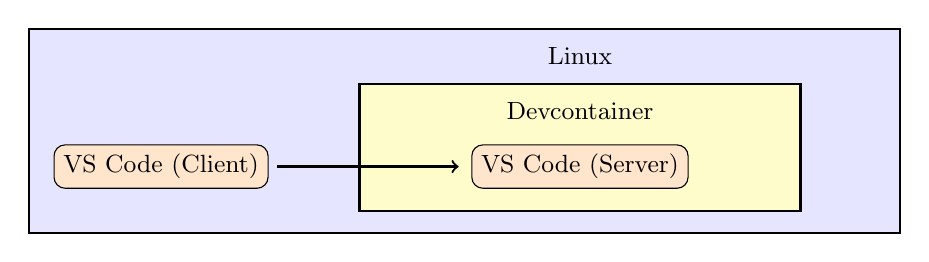
\begin{tikzpicture}[scale=1.4, every node/.style={font=\small}]
      % Linux box
      \draw[thick, fill=blue!10] (-2,0.4) rectangle (5.9,2.25);
      \node at (3,2) {Linux};
      % Devcontainer box inside WSL2 distro
      \draw[thick, fill=yellow!20] (1,0.6) rectangle (5,1.75);
      \node at (3,1.5) {Devcontainer};
      % VS Code Server box inside WSL2 distro
      \node[draw, fill=orange!20, rounded corners] at (3,1) {VS Code (Server)};
      % VS Code (Client) outside, arrow to Devcontainer
      \node[draw, fill=orange!20, rounded corners] at (-0.8,1) {VS Code (Client)};
      \draw[->, thick] (0.25,1) -- (1.9,1);
    \end{tikzpicture}
    \caption{Devcontainer-ak Linux-en}
  \end{figure}
\end{frame}

\begin{frame}
  \frametitle{Zer da Devcontainer bat?}
  \begin{itemize}
    \item VS Code-ren zerbitzari zatia Container \textbf{barruan} exekutatzen da.
    \item Garatzailea bere sistema eragilean duen VS Code-rekin konektatu daiteke bezero gisa. Horrela, \textbf{garapena Container-ean} egon balitz bezala egiten da.
  \end{itemize}
  \begin{figure}
    \centering
    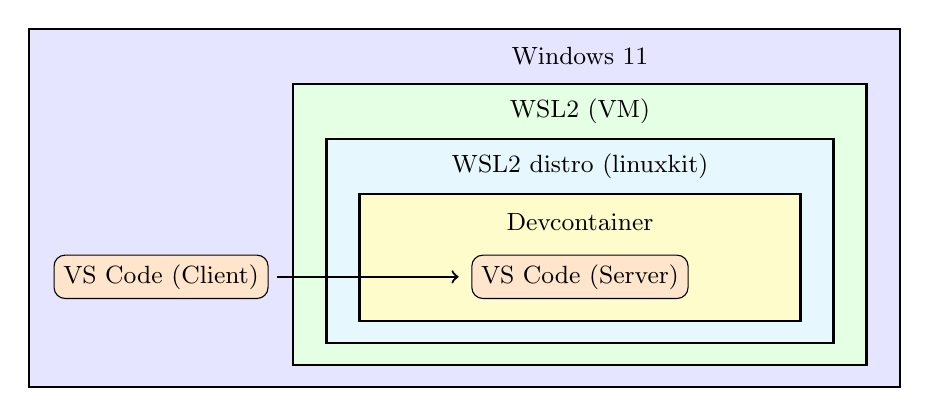
\begin{tikzpicture}[scale=1.4, every node/.style={font=\small}]
      % Windows box
      \draw[thick, fill=blue!10] (-2,0) rectangle (5.9,3.25);
      \node at (3,3) {Windows 11};
      % WSL2 (VM) box inside Windows
      \draw[thick, fill=green!10] (0.4,0.2) rectangle (5.6,2.75);
      \node at (3,2.5) {WSL2 (VM)};
      % WSL2 distro box inside WSL2 (VM)
      \draw[thick, fill=cyan!10] (0.7,0.4) rectangle (5.3,2.25);
      \node at (3,2) {WSL2 distro (linuxkit)};
      % Devcontainer box inside WSL2 distro
      \draw[thick, fill=yellow!20] (1,0.6) rectangle (5,1.75);
      \node at (3,1.5) {Devcontainer};
      % VS Code Server box inside WSL2 distro
      \node[draw, fill=orange!20, rounded corners] at (3,1) {VS Code (Server)};
      % VS Code (Client) outside, arrow to Devcontainer
      \node[draw, fill=orange!20, rounded corners] at (-0.8,1) {VS Code (Client)};
      \draw[->, thick] (0.25,1) -- (1.9,1);
    \end{tikzpicture}
    \caption{Devcontainer-ak Windows-en}
  \end{figure}
\end{frame}

\begin{frame}
  \frametitle{Zer da Devcontainer bat?}
  \begin{itemize}
    \item Hasieran Microsoftek bultzatu zuen baina orain espezifikazio \textbf{ireki} bat da:
      \url{https://containers.dev/}
    \item Devcontainer-ak \textbf{Docker} edo \textbf{Podman} bezalako \textbf{OCI} (\textit{Open Container Initiative}) konteinerrak erabiltzen ditu.
    \item Ez dago VS Code-i lotuta. \textbf{Jetbrains-ek} ere eskaintzen du Devcontainer-ak erabiltzeko modua: \url{https://www.jetbrains.com/remote-development/gateway/}
  \end{itemize}
\end{frame}

\begin{frame}
  \frametitle{Garrantzia graduan}
  \begin{itemize}
    \item Ikasleek eta irakasleek \textbf{hainbat} garapen-ingurune erabili behar dituzte gradu osoan zehar. Ikasgai ezberdinak, transferentzia proiektuak, ikerketa, ...
    \item Devcontainer-ek ingurune hauek elkarren artean \textbf{bereizten} laguntzen dute.
      \begin{itemize}
        \item Bertsio ezberdinen arteko \textbf{talkak ekiditen} laguntzen dute.
      \end{itemize}
    \item Devcontainer-ek garapen ingurunea gure sistema eragiletik (\textit{host-etik}) bereizten laguntzen dute. \textbf{Ez dute gure SEa aldatzen}.
    \item \textbf{Erreplikagarriak} dira. Ikasleek eta irakasleek ingurune berdina izan dezaten laguntzen dute.
  \end{itemize}
\end{frame}

\begin{frame}
  \frametitle{Demo time!}
\end{frame}

\section{Gure esperientzia}

\begin{frame}
  \frametitle{Zer egin dugu?}
  \begin{itemize}
    \item Devcontainer-ei buruzko \textbf{git biltegi} bat sortu dugu:
      \url{https://gitlab.com/mu-bd-ce/devcontainers}.

      Bertan aurkituko ditugu:
      \begin{itemize}
        \item Programazio lengoaia ezberdinendako \textbf{aurrez-sorturiko Devcontainer-ak}. Adibidez:
          \url{registry.gitlab.com/mu-bd-ce/devcontainers/python:latest}
        \item Hauei buruzko \textbf{dokumentazioa}:
          \url{https://mu-bd-ce.gitlab.io/devcontainers}
        \item Hauek nola erabili azaltzen duten \textbf{adibideak}.
      \end{itemize}
    \item Bigarren mailako Web eta Estatistika ikasgaietan \textbf{lehenengo saiakera} egin dugu.
  \end{itemize}
\end{frame}

\subsection{The good, the bad and the ugly}

\begin{frame}
  \frametitle{The good}
  \begin{columns}
    \begin{column}{0.7\linewidth}
      \begin{itemize}
        \item Web eta Estatistika ikasgaietako garapen inguruneak container barruan sartzea lortu dugu.
        \item Kontrol puntuetan ez dugu aparteko arazorik izan.
        \item PBL-an:
          \begin{itemize}
            \item Ikasleek Devcontainer-ak erabili dituzte, eta nahiko \textbf{autonomoak} izan dira.
            \item \textbf{Docker Compose} erabiliz, Datu Basea eta backend aplikazioa garatu dituzte.
          \end{itemize}
        \item Errendimendua:
          \begin{itemize}
            \item Linuxen Devcontainer-en \textbf{errendimendua} oso ona da.
            \item Windowsen, makina birtual bat izan arren, WSL2-ren errendimendua nahiko ona da \textbf{CPU} erabilerari dagokionez.
          \end{itemize}
      \end{itemize}
    \end{column}
    \begin{column}{0.25\linewidth}
      \begin{figure}
        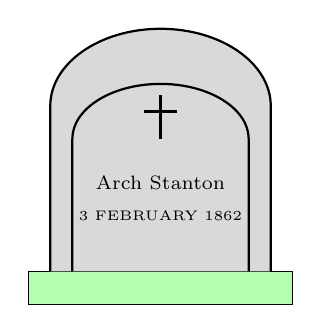
\begin{tikzpicture}[scale=1.4]
          % Ground
          \draw[fill=green!30] (-0.2,0.2) rectangle (2.2,0.5);
          % Grave
          \draw[thick, fill=gray!30] (0,0.5) -- (0,2) arc (180:0:1 and 0.7) -- (2,0.5);
          \draw[thick] (0.2,0.5) -- (0.2,1.7) arc (180:0:0.8 and 0.5) -- (1.8,0.5);
          % R.I.P. text
          \node at (1,1.3) {\scriptsize Arch Stanton};
          \node at (1,1) {\tiny 3 FEBRUARY 1862};
          % Cross
          \draw[thick] (1,1.7) -- (1,2.1);
          \draw[thick] (0.85,1.95) -- (1.15,1.95);
        \end{tikzpicture}
        \caption{Arch Stanton-en hilobia (Altxorra ez dago hemen)}
      \end{figure}
    \end{column}
  \end{columns}
\end{frame}

\begin{frame}
  \frametitle{The bad}
  \begin{itemize}
    \item Windows-en \textbf{I/O errendimendua} ez da ona. Batez ere Lan-eremuko\\(``workspace''-ko) fitxategietan sarrera/irteera operazio asko egiten badira.
    \item Windows eta Linuxeko fitxategi sistemen arteko \textbf{baimenak} arazoak.
  \end{itemize}
  \begin{figure}
    \centering
    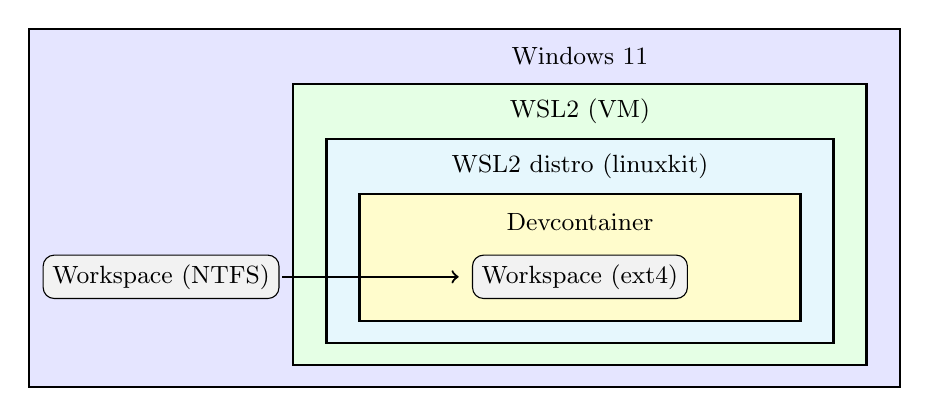
\begin{tikzpicture}[scale=1.4, every node/.style={font=\small}]
      % Windows box
      \draw[thick, fill=blue!10] (-2,0) rectangle (5.9,3.25);
      \node at (3,3) {Windows 11};
      % WSL2 (VM) box inside Windows
      \draw[thick, fill=green!10] (0.4,0.2) rectangle (5.6,2.75);
      \node at (3,2.5) {WSL2 (VM)};
      % WSL2 distro box inside WSL2 (VM)
      \draw[thick, fill=cyan!10] (0.7,0.4) rectangle (5.3,2.25);
      \node at (3,2) {WSL2 distro (linuxkit)};
      % Devcontainer box inside WSL2 distro
      \draw[thick, fill=yellow!20] (1,0.6) rectangle (5,1.75);
      \node at (3,1.5) {Devcontainer};
      % VS Code (Client) outside, arrow to Devcontainer
      % VS Code Server box inside WSL2 distro
      \node[draw, fill=gray!10, rounded corners] at (3,1) {Workspace (ext4)};
      \node[draw, fill=gray!10, rounded corners] at (-0.8,1) {Workspace (NTFS)};
      \draw[->, thick] (0.3,1) -- (1.9,1);
    \end{tikzpicture}
    \caption{``Reopen in container'' era}
  \end{figure}
\end{frame}

\begin{frame}
  \frametitle{The ugly: Konponbideak}
  \begin{itemize}
    \item Sarrera/irteera asko duten fitxategiak lan eremutik ateratzea: Konpilatzeko edo exekutatzeko erabiltzen diren fitxategiak (gure proiektuaren iturria osatzen ez dutenak) lan-eremutik ateratzea \textbf{gomendatzen da}. Horrela, errendimendu arazoak saihesten dira.
  \end{itemize}
\end{frame}

\begin{frame}
  \frametitle{The ugly: Konponbideak}
  \begin{itemize}
    \item Lan eremua WSLko beste distribuzio batean izatea: Ikus: \url{https://gitlab.com/mgep-web-ingeniaritza-1/pbl/spring-devcontainer-kaixo-mundua\#handitu-abiadura-windows-en}
  \end{itemize}
  \begin{figure}
    \centering
    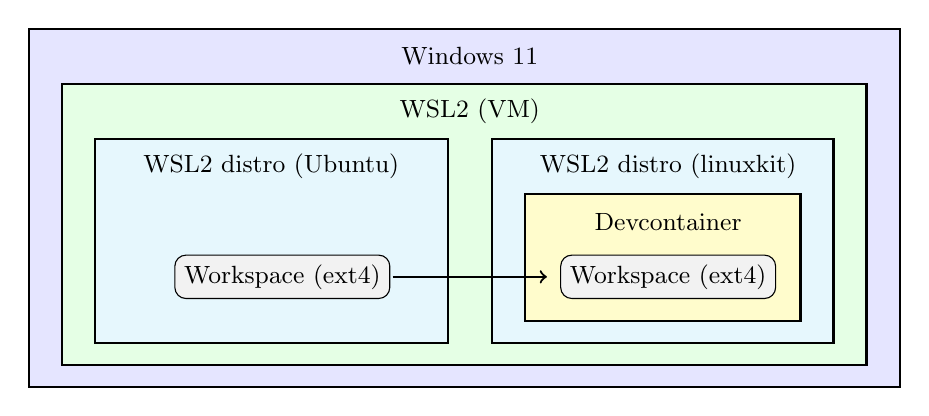
\begin{tikzpicture}[scale=1.4, every node/.style={font=\small}]
      % Windows box
      \draw[thick, fill=blue!10] (-2,0) rectangle (5.9,3.25);
      \node at (2,3) {Windows 11};
      % WSL2 (VM) box inside Windows
      \draw[thick, fill=green!10] (-1.7,0.2) rectangle (5.6,2.75);
      \node at (2,2.5) {WSL2 (VM)};
      % WSL2 distro box inside WSL2 (VM)
      \draw[thick, fill=cyan!10] (-1.4,0.4) rectangle (1.8,2.25);
      \node at (0.2,2) {WSL2 distro (Ubuntu)};
      % WSL2 distro box inside WSL2 (VM)
      \draw[thick, fill=cyan!10] (2.2,0.4) rectangle (5.3,2.25);
      \node at (3.8,2) {WSL2 distro (linuxkit)};
      % Devcontainer box inside WSL2 distro
      \draw[thick, fill=yellow!20] (2.5,0.6) rectangle (5,1.75);
      \node at (3.8,1.5) {Devcontainer};
      % VS Code Server box inside WSL2 distro
      \node[draw, fill=gray!10, rounded corners] at (3.8,1) {Workspace (ext4)};
      \node[draw, fill=gray!10, rounded corners] at (0.3,1) {Workspace (ext4)};
      \draw[->, thick] (1.3,1) -- (2.7,1);
    \end{tikzpicture}
    \caption{WSL era}
  \end{figure}
\end{frame}

\begin{frame}
  \frametitle{The ugly: Konponbideak}
  \begin{itemize}
    \item ``Clone Repository in Container Volume'' era.
  \end{itemize}

  \begin{figure}
    \centering
    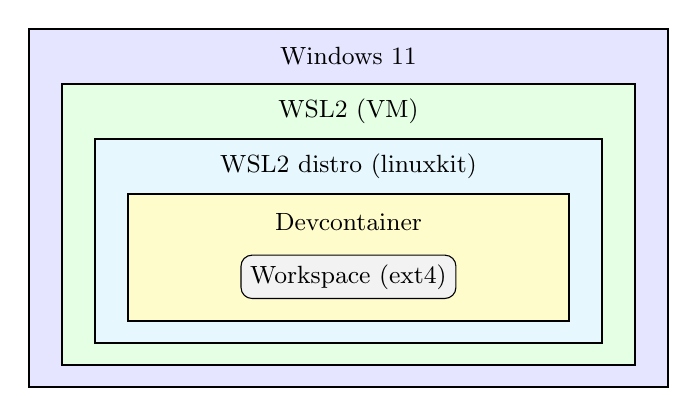
\begin{tikzpicture}[scale=1.4, every node/.style={font=\small}]
      % Windows box
      \draw[thick, fill=blue!10] (0.1,0) rectangle (5.9,3.25);
      \node at (3,3) {Windows 11};
      % WSL2 (VM) box inside Windows
      \draw[thick, fill=green!10] (0.4,0.2) rectangle (5.6,2.75);
      \node at (3,2.5) {WSL2 (VM)};
      % WSL2 distro box inside WSL2 (VM)
      \draw[thick, fill=cyan!10] (0.7,0.4) rectangle (5.3,2.25);
      \node at (3,2) {WSL2 distro (linuxkit)};
      % Devcontainer box inside WSL2 distro
      \draw[thick, fill=yellow!20] (1,0.6) rectangle (5,1.75);
      \node at (3,1.5) {Devcontainer};
      % VS Code (Client) outside, arrow to Devcontainer
      % VS Code Server box inside WSL2 distro
      \node[draw, fill=gray!10, rounded corners] at (3,1) {Workspace (ext4)};
    \end{tikzpicture}
    \caption{``Clone Repository in Container Volume'' era}
  \end{figure}
\end{frame}

\section{Eztabaida}

\begin{frame}
  \frametitle{Gure Proposamena}
  \begin{itemize}
    \item Hurrengo kurtsoan ekimen honetara \textbf{ikasgai gehiago batzea}.
    \item Git biltegia graduan erabiltzen ditugun \textbf{teknologiak estandarizatzeko} erabiltzea (adibidez, graduko Java bertsioa) \footnote{Biltegi hau lehenengo hurbilketa da; Devcontainer hauen alderdi guztiak eztabaidatzeko \textbf{irekita} daude.}.
  \end{itemize}

\end{frame}

\section[Three more things...]{Gehigarriak}

\begin{frame}
  \frametitle{Github Codespaces}
  \begin{itemize}
    \item Devcontainer-ak \textbf{GitHub Codespaces}-en erabil daitezke.
    \item Codespace bat urruneko container bat da, GitHub-eko zerbitzarietan exekutatzen dena.
    \item Bertara konektatzeko, \textbf{VS Code} bezeroa edo \textbf{Web} bezeroa erabil daiteke.
  \end{itemize}
\end{frame}

\begin{frame}
  \frametitle{MU LaTeX template}
  \begin{itemize}
    \item Mondragon Unibertsitateko estilo jarraibideak betetzen dituzten LaTeX klaseen bilduma eskaintzen du.
    \item Klaseek hainbat dokumentu mota onartzen dituzte, besteak beste:
      \begin{itemize}
        \item Liburuak (\textbf{mubook})
        \item Azterketak (\textbf{mutest})
        \item Aurkezpenak (\textbf{mupresentation})
      \end{itemize}
    \item LaTeX-eko devcontainer-ak txantiloi hauek instalatuta ditu jada, zuzenean erabiltzeko prest.
    \item Ikus: \url{https://gitlab.com/mu-bd-ce/mu-latex-template}
  \end{itemize}
\end{frame}

\begin{frame}
  \frametitle{Github Copilot}
  \begin{itemize}
    \item Devcontainer-etan \textbf{Github Copilot} erabil daiteke.
    \item Github Copilot-ek \textbf{GPT-4.1} eta \textbf{GPT-4o} dohainik eskaintzen ditu.
    \item Github Education-ek \textbf{Premium modeloak} eskaintzen ditu (Claude Sonnet 4, ...).
  \end{itemize}
\end{frame}

\muback{Eskerrik asko}{Ibai Roman\\
  Software \& System Engineering\\
  Electronics and Computer Science department\\
  Mondragon Unibertsitatea - Faculty of Engineering\\
\href{www.mondragon.edu}{www.mondragon.edu}}

\end{document}